\documentclass{article}
\usepackage{amsmath, amssymb}
\usepackage{tikz}
\usetikzlibrary{arrows.meta}

\begin{document}

\begin{figure}[h]
    \centering
    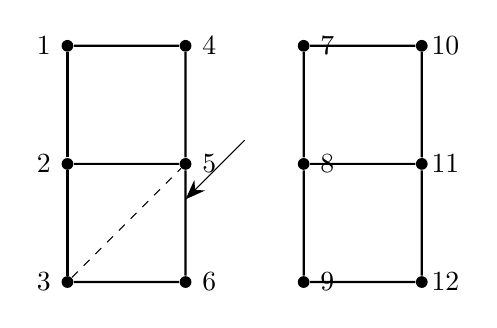
\begin{tikzpicture}[scale=1.5]
        % Draw the graph with labeled vertices
        \node[circle,fill,inner sep=1.5pt,label={0:}] (1) at (0,3) {};
        \node[circle,fill,inner sep=1.5pt,label={0:}] (2) at (0,2) {};
        \node[circle,fill,inner sep=1.5pt,label={0:}] (3) at (0,1) {};
        \node[circle,fill,inner sep=1.5pt,label={0:}] (4) at (1,3) {};
        \node[circle,fill,inner sep=1.5pt,label={0:}] (5) at (1,2) {};
        \node[circle,fill,inner sep=1.5pt,label={0:}] (6) at (1,1) {};
        \node[circle,fill,inner sep=1.5pt,label={0:}] (7) at (2,3) {};
        \node[circle,fill,inner sep=1.5pt,label={0:}] (8) at (2,2) {};
        \node[circle,fill,inner sep=1.5pt,label={0:}] (9) at (2,1) {};
        \node[circle,fill,inner sep=1.5pt,label={0:}] (10) at (3,3) {};
        \node[circle,fill,inner sep=1.5pt,label={0:}] (11) at (3,2) {};
        \node[circle,fill,inner sep=1.5pt,label={0:}] (12) at (3,1) {};
        
        \node at (-0.2,3) {1};
        \node at (-0.2,2) {2};
        \node at (-0.2,1) {3};
        \node at (1.2,3) {4};
        \node at (1.2,2) {5};
        \node at (1.2,1) {6};
        \node at (2.2,3) {7};
        \node at (2.2,2) {8};
        \node at (2.2,1) {9};
        \node at (3.2,3) {10};
        \node at (3.2,2) {11};
        \node at (3.2,1) {12};
        
        % Draw the edges
        \draw[thick] (1) -- (2);
        \draw[thick] (2) -- (3);
        \draw[thick] (4) -- (5);
        \draw[thick] (5) -- (6);
        \draw[thick] (7) -- (8);
        \draw[thick] (8) -- (9);
        \draw[thick] (10) -- (11);
        \draw[thick] (11) -- (12);
        \draw[thick] (1) -- (4);
        \draw[thick] (2) -- (5);
        \draw[thick] (3) -- (6);
        \draw[thick] (7) -- (10);
        \draw[thick] (8) -- (11);
        \draw[thick] (9) -- (12);
        
        % Draw the dashed edge
        \draw[dashed] (3) -- (5);
        
        % Add the arrow indicating the transformation
        \draw[-{Stealth[scale=1.5]}] (1.5, 2.2) -- ++(-0.5, -0.5);
    \end{tikzpicture}
    \caption{Non-symmetric space with $N=3$, $L_*=4$. The dashed line indicates an edge that can be added or removed while maintaining the $L_*$-uniform scaling property as per Definition \ref{def:removable}. Any edge connecting vertically aligned points is removable in this context.}
    \label{fig:non_symmetric_space}
\end{figure}

\end{document}